%!TEX root = ../bachelorthesis.tex


\chapter{Einleitung}
\markboth{Einleitung}{}
\label{sec:Einleitung}
\section{Kontext}
Im Rahmen des Studiums der Sozialinformatik wurde in der \ac{kita} \textit{Schloss Ardeck} in Gau-Algesheim vom Autor dieser Arbeit ein lokales soziales Netzwerk als Kommunikations- und Dokumentenmanagementsystem eingeführt. In dem \textit{KitaNet} genannten System können durch die Leitung und Mitarbeitenden der Einrichtung beispielsweise Elternbriefe ausgetauscht und erarbeitet werden oder Terminabsprachen und Diskussionen geführt werden, auch wenn die Kolleginnen aufgrund von Schichtdiensten nicht immer direkten Kontakt haben. \\ Das Projekt wurde innerhalb von zwei Jahren realisiert und in der \ac{kita} implementiert.

Technisch besteht KitaNet aus einer \ac{vm} auf einem NAS-System der Firma QNAP. Auf der \ac{vm} läuft die auf der Skriptsprache \ac{php} basierende Software \textit{HumHub}. Diese arbeitet mit einer durch QNAP bereitgestellten Variante eines \ac{ldap} zur Benutzerverwaltung zusammen. Dies war notwendig, um der Leitung der Kita eine Möglichkeit zu bieten, Nutzerpasswörter grundzustellen und neue Nutzer anzulegen. Gerade das Grundstellen von Passwörtern ist in der täglichen Arbeit leider häufiger notwendig, als von den Projektdurchführenden geplant und bindet somit einen nicht unerheblichen Teil der Arbeitszeit der Leitung.

HumHub selbst bietet die Möglichkeit, beim Nutzer eine E-Mail-Adresse zu hinterlegen, über die dann ein Grundstellen des Passwortes möglich ist. Hierfür wäre allerdings ein E-Mail-Server innerhalb des Netzwerkes notwendig. Diese Funktion wurde im Rahmen des IT-Projektes nicht genutzt. Im Rahmen dieser Bachelorarbeit soll nun der Frage nachgegangen werden, wie die Implementierung eines Mailservers in die Umgebung aus \ac{vm}, \ac{ldap} und HumHub durchgeführt werden kann. Hierfür soll die in der \ac{kita} vorliegende Umgebung auf einem separaten Server nachgestellt werden, um den Produktivbetrieb in der \ac{kita} nicht zu gefährden.

\section{Aufbau und Gestaltung der Arbeit}

In dieser Bachelor-Thesis soll zunächst KitaNet sowie die hier vorliegende Hardwareumgebung und das Einsatzszenario erläutert werden. Hier sollen auch Hinderungsgründe genannt werden, die eine Umsetzung der in dieser Thesis beschriebenen Lösung in den Produktivbetrieb der Kita verhindern. In diesem Kapitel wird auch die Funktionalität eines \ac{ldap} beschrieben.

Das nächste Kapitel behandelt zunächst die Funktionsweise eines \ac{smtp}-Servers. Im Anschluss werden die Anforderungen und Nutzungsszenarien des Mailservers für KitaNet festgelegt. Die Anforderungen umfassen dabei zum Einen Punkte wie die Zusammenarbeit mit einem Nutzerverzeichnis, verbunden mit einer möglichen Automation des Anlegens von Mail-Nutzern, sollen aber zum Anderen auch nichtfunktionale Aspekte, wie den zu erwartenden Pflegeaufwand oder die finanzielle Belastung durch etwaige Lizenzkosten, beachten.

Die benannten Nutzungsszenarien bilden die Grundlage zur Formulierung von Tests, die die Funktionalität und Praxistauglichkeit der späteren Installation sicherstellen sollen. Die Beschreibung dieser Tests bildet den Abschluss  dieses Kapitels.

Anschließend werden die zur Wahl stehenden Softwarepakete \textit{postfix} und die kommerzielle Software \textit{EmailSuccess} vorgestellt. Die im vorherigen Kapitel formulierten Anforderungen werden mit dem Funktionsumfang der Softwarepakete abgeglichen. Aufgrund der Ergebnisse dieses Abgleichs erfolgt die Entscheidung. 

Dessen Installation bildet das nächste Kapitel. Es wird dargestellt, ob und welche Anpassungen durchzuführen sind, um den \ac{smtp}-Server in die vorliegende Umgebung zu integrieren. Auch die Anbindung an das \ac{ldap} wird beschrieben.
Die Dokumentation der durchgeführten Tests schließt das Kapitel ab. An dieser Stelle soll auch kritisch hinterfragt werden, ob die im Vorfeld formulierten Tests ausreichend spezifisch waren oder Anpassungen an diesen vorzunehmen waren.

Ein persönliches Fazit schließt diese Bachelor-Thesis ab.

\textit{Erstmalige Fachbegriffe oder Eigennamen } werden \textit{kursiv} dargestellt und in diesem Kontext erläutert.  \\ \textquote{Zitate werden mit französischen Anführungszeichen gekennzeichnet}. \\ \verb+Code oder ähnliches+ wiederum werden immer in einer \verb+Monospace-Schriftart+ ausgegeben, um ihn vom umliegenden Text zu separieren. \\ Abkürzungen und Akronyme wie \zb \ac{nas} werden bei der ersten Erwähnung kursiv ausgeschrieben und mit der Abkürzung benannt. Diese findet sich dann auch im Abkürzungsverzeichnis. Im weiteren Text erscheinen Sie nur noch abgekürzt. 

\section{Methodik}

Wie im vorherigen Abschnitt beschrieben, erfolgt die Auswahl der zu installierenden Software aufgrund des Abgleichs mit zuvor festgelegten Anforderungen.

Hierzu werden die Angaben des jeweiligen Herstellers, respektive bei nicht kommerzieller Software der Projektverantwortlichen, herangezogen um eine objektive Vergleichbarkeit der Softwareprodukte sicherzustellen. Die Entscheidung wird somit grundsätzlich aufgrund objektiver Grundlagen getroffen.  Da beispielsweise die finanzielle Situation der \ac{kita} nur einen geringen Spielraum für Investitionen zulässt, können die formulierten Anforderungen nicht vollständig gleichwertig behandelt werden. Werden Anforderungen, \zb aufgrund wirtschaftlicher Erwägungen, unterschiedlich gewichtet, wird dies gesondert im Text erwähnt.

Es findet somit eine Mischung aus qualitativer und quantitativer Forschung statt.

Die Implementierung erfolgt anschließend im Rahmen eines Experiments in einer KitaNet nachempfunden Umgebung statt.

Die Funktionsweise von KitaNet und sein Nutzen für die \ac{kita} sollen im nächsten Kapitel erläutert werden.

\chapter{KitaNet}

%Kurze Beschreibung von technischer Basis von KitaNet. Was sind soziale Netzwerke?
%Ablauf beim Grundstellen von Passwörtern wird erläutert.

KitaNet ist der Arbeitstitel eines IT-Projektes, das im Rahmen des Studiums der Sozialinformatik vom Autor dieser Thesis mit einem Kommilitonen durchgeführt wurde. Hierfür wurde in Zusammenarbeit mit der \ac{kita} Schloss Ardeck in Gau-Algesheim ein soziales Netzwerk installiert, über welches die Bediensteten der Kita eine Plattform zum Austausch und Kommunikation erhalten. 

Die \ac{kita} betreut ca. 170 Kinder im Alter von einem bis sechs Jahren. Hierfür beschäftigt sie 30 pädagogische Fachkräfte, welche die ihnen anvertrauten Kinder in acht Gruppen betreuen. Die Kita befindet sich in kommunaler Trägerschaft \citep[vgl.][]{kitaweb}.

Für die Umsetzung der Idee eines sozialen Netzwerkes konnten die Studenten unter anderem von dem Umstand profitieren, dass jede Gruppe der Kita mit Notebooks ausgestattet ist, über welche die Kinder Lernspiele spielen, aber auch unter Betreuung der Erzieher erste Erfahrungen mit dem Internet sammeln.

Die technische Umgebung in der Kita, sowie die Umsetzung des sozialen Netzwerks sollen nun genauer beschrieben werden. Auch sollen hier Unterschiede zur Testumgebung dieser Bachelor-Arbeit aufgezeigt werden.

\section{Hardware}
%Beschreibt den technischen Aufbau von KitaNet in der Kita selbst.
%Abweichungen vom Aufbau für Studienprojekt werden erläutert. Was weicht ab?
%Verhindert die für dieses Bachelorarbeit eingesetzte Hardware eine Umsetzung in der Kita?
In der \ac{kita} wurde im Rahmen einer Elterninitiative ein lokales Netzwerk bestehend aus fünf WLAN-Routern installiert. Dieses \ac{lan} vernetzt nicht nur die vier Gebäudeteile der Kita miteinander, es stellt zugleich die telefonische Erreichbarkeit der einzelnen Gruppen sicher. Dieses Netzwerk wurde in der Vergangenheit unter anderem dazu genutzt, Dokumente am zentralen Netzwerkdrucker im Büro der Leitung auszudrucken.

Die Studierenden entschieden sich zur Umsetzung des Projektes KitaNet für die im Anschluss näher erläuterte Software HumHub.
Einer der Vorteile war, dass diese kostenlos auf einem privaten Server installiert werden konnte. Die Installation erfolgte auf einem \ac{nas} der Firma \textit{QNAP}, genauer einem QNAP TS-253B \citep[vgl.][]{qnap}. Im von der Verwaltungssoftware des \ac{nas} bereitgestellten \textit{VM-Manager} wurde ein virtueller Ubuntu-Server erstellt, auf dem die Software Humhub installiert wurde.

Im Vergleich zum Produktivaufbau ergibt sich hier der erste Unterschied zum Versuchsaufbau für diese Arbeit. Anstatt einen Ubuntu-Server als virtuelle Maschine in einem \ac{nas} aufzusetzen, wird hier der Server auf echter Hardware betrieben. 

Die Nutzung einer \ac{vm} im Rahmen des Projektes war damit begründet, dass die Softwareinstallation auf dem NAS selbst nur in einem engen Rahmen möglich war. Die Nutzung einer Ubuntu-VM ermöglichte es den Studenten, die Installation in einer standardisierten Umgebung vornehmen zu können, ohne etwaige Besonderheiten des QNAP-Betriebssystems berücksichtigen zu müssen.

Im Rahmen dieser Bachelorarbeit wird, wie eingangs beschrieben, die Produktivumgebung bestmöglich nachgebildet. Hierfür dient ein Fujitsu Esprimo C5730 E als Hardware, auf der Ubuntu 20.04 LTS als Betriebssystem installiert wurde. Nach Ansicht des Autors hat die verwendete Hardware keine nennenswerte Auswirkung auf die Funktionalität des beschriebenen Versuchsaufbaus. \\ Einzige zu beachtende Besonderheit ist, dass das später beschriebene \ac{ldap} in der Produktivumgebung nicht auf der \ac{vm} sondern auf dem \ac{nas} selbst ausgeführt wird. Hier wäre die Konfiguration für eine Übernahme ins Produktivsystem entsprechend anzupassen.

Wie bereits erwähnt kommt innerhalb der \ac{vm} die Software HumHub zum Einsatz. Der Umfang und die Funktionen dieser Software soll nun kurz erläutert werden.

\section{HumHub}

Bei ihren Recherchen für die Umsetzung des IT-Projektes stießen die Studenten auf die Social-Network-Software HumHub. Die Software ist quelloffen und wird von der HumHub GmbH \& Co.KG aus München vertrieben. Die Möglichkeit, die Software kostenlos für nicht kommerzielle Zwecke installieren und betreiben zu können, gab letztlich den Ausschlag für Entscheidung  \textquote{HumHub ist eine freie und sehr flexible Social Networking Software, die auf eigenen Servern gehosted werden kann} \citep{humhubmain}.

Die Grundfunktionen von HumHub und die Möglichkeit der Erweiterung der Grundfunktionen soll im Weiteren betrachtet werden.

\subsection{Spaces}

Spaces geben HumHub seine Grundstruktur. \textquote{A space serves as an independent area within your network with an own set of members, permissions, settings and modules} \citep{spaces}. 
Eine Nutzerin kann Mitglied mehrerer Spaces sein und innerhalb der Spaces verschiedene Rollen einnehmen. Diese reichen von \textit{Besitzer} des Spaces, der nahezu volle Kontrolle über sämtliche Nutzer und Beiträge innerhalb des jeweiligen Spaces hat, über den \textit{Moderator} der Beiträge verwalten kann, bis hin zum normalen Mitglied, das Beiträge erstellen kann, wenn dies vom Besitzer erlaubt wurde.  

Zentraler Sammelpunkt für Beiträge ist der Stream, dessen Inhalt sich je nach Kontext verändert. Betrachtet ein Nutzer seine Startseite, werden ihm sämtliche Beiträge aus all seinen Spaces angezeigt. Befindet er sich in einem Space, sind nur dort erstellte Beiträge sichtbar.

Mit den Spaces bietet Humhub die Möglichkeit, Gruppenstrukturen abzubilden. Jedoch kann in den Gruppen nicht viel mehr getan werden, als Bilder oder Texte zu erstellen und diese zu kommentieren.
Sein volles Potential kann Humhub mit den Möglichkeiten entfalten, Module zur Funktionserweiterung nachzuladen.

\subsection{Module}

\textquote{The feature set of your HumHub network can be extended by installing additional modules} \citep[][]{modules}. Zur Erweiterung der Funktionalität stehen diverse Module wie Kalender, Dateiablage, Abstimmungen oder ein Wiki zur Verfügung.
Module können für einzelne Spaces aktiviert werden, um den Bedürfnissen des jeweiligen Kontext gerecht zu werden \citep[vgl.][ff.]{modules}. Ein Space, der zur Organisation des Sommerfestes der Kita eingerichtet wurde, benötigt \zb in der Regel keinen Kalender, sehr wohl aber eine Dateiablagestruktur.
So wird der einzelne Space nicht mit unnötigen Features überladen, die vom Zweck der Umgebung ablenken würden.

Besondere Erwähnung sollte die Erweiterung \textit{Ankündigungen} erhalten. 
Eine Ankündigung wird im Stream des Spaces grundsätzlich wie eine einfache Mitteilung angezeigt. Einzige Besonderheit ist, dass die Nutzer den Post mit einem Klick zur Kenntnis nehmen können. Diese Kenntnisnahme kann dann vom Ersteller des Beitrags oder einem Moderator \zb als Excel-Datei exportiert werden  \citep[Quellcode unter][]{announcement}. Da dieser Mitteilung auch Dateien angehängt werden können, konnten die Studenten die Forderung der Leitung nach Protokollierung der Einsichtnahme von Dokumenten Rechnung tragen.


\section{LDAP}

Zum Anlegen der Benutzer innerhalb des KitaNet wurde die Benutzerverwaltung des QNAP-NAS auf Basis von LDAP genutzt. Die Funktionsweise von LDAP soll daher ebenfalls kurz erläutert werden.

\subsection{Funktionsweise und Datenmodell}

Ein \ac{ldap} stellt eine zentrale Verwaltung innerhalb eines Netzwerkes dar.
\textquote{Verzeichnisdienste wie \textquote{OpenLDAP} ermöglichen es Ihnen, die Verwaltung der Ressourcen zentral zu steuern und an mehreren Stellen zu replizieren} \citep[][611]{Deimeke2019}. 

\ac{ldap} besteht jedoch nicht nur aus einer Datenbank, sondern beinhaltet zugleich auch ein passendes Netzwerkprotokoll, um mit der Datenbank interagieren zu können \citep[vgl.][3]{Gietz}.

Deimeke \ua führen weiter aus, dass der Vorteil des Einsatzes eines \ac{ldap} darin besteht, dass jeder Nutzer nur noch ein Konto besitzt, dessen Passwort dann zentral verwaltet und geändert werden kann. \textquote{Um diese zentrale Verwaltung der Ressourcen realisieren zu können, wurde das \textit{Lightweight Directory Access Protocol} (LDAP) entwickelt} \citep[][611]{Deimeke2019}.

Innerhalb des \ac{ldap} werden die Daten zu den einzelnen Ressourcen innerhalb einer Hierarchie, dem \ac{dit} abgelegt \citep[vgl.][7]{rfc4512}. Zentraler Inhalt des \ac{dit} bilden Objekte. Diese sind die zu verwaltenden Ressourcen \citep[vgl.][614]{Deimeke2019}. \textquote{Ein Objekt kann sowohl ein Container sein, in dem weitere Objekte verwaltet werden, als auch ein Benutzer oder eine Gruppe sein. Eines ist bei allen Objekten aber immer gleich: Alle Objekte haben Eigenschaften, die \textit{Attribute}} \citep[][614]{Deimeke2019}. Eines dieser Attribute ist \zb die \textit{uid}, welche den Login-Namen des Nutzers repräsentiert \citep[][18]{rfc4519}. \\ Innerhalb der Baumstruktur des \ac{dit} bilden die Nutzer die Blätter. Davon abgegrenzt werden die Äste. Diese werden von Containerobjekten gebildet, welche man auch als \ac{ou} bezeichnet \citep[vgl.][614]{Deimeke2019}.

Angesprochen werden diese Objekte über seinen \ac{dn}, einen für jedes Objekt eindeutigen Namen, vergleichbar mit dem in Dateisystemen geläufigen Prinzip von Dateipfad und Dateinamen (\zb \verb+C:/Ordner/Datei.txt+) \citep[vgl.][613]{Deimeke2019}. 

Die Mitgliedschaft der Blatt-Objekte in Gruppen kann über Suchanfragen an \ac{ldap} ausgelesen werden. Beispielsweise gibt die Suchanfrage \verb+ldapsearch -x  "(uid=admin)"+ in der Konsole eines Servers den Eintrag im \ac{ldap} zurück, der den Login-Namen \textit{admin} besitzt.

Wie HumHub \bzw KitaNet nun mit dem \ac{ldap} zusammenarbeiten, soll im nächsten Abschnitt an ausgewählten Beispielen erläutert werden.

\subsection{LDAP und HumHub}

Innerhalb von HumHub kann die \ac{ldap}-Anbindung über das Webinterface konfiguriert werden \citep[vgl.][]{humldap}. Die nachfolgenden Abbildungen zeigen die Eingaben in der Testumgebung. 

\begin{figure}[h]
  \centering
  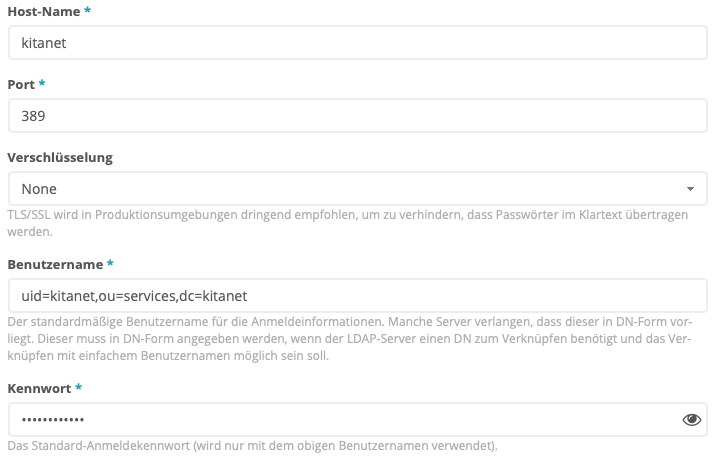
\includegraphics[width=1.0\textwidth]{res/ldapkitanet1.png}
  \caption{Teil 1 der LDAP-Konfiguration für Kitanet (Eigene Abbildung)}
  \label{fig:LDAP Kitanet Teil 1}
\end{figure}

In der Zeile \textit{Benutzername} ist ein Beispiel für eine \ac{dn} zu sehen. Für den Login im LDAP wird der Nutzer mit dem \ac{cn} \textit{admin} in dem \ac{dc} \textit{kitanet} verwendet.

\begin{figure}[h]
  \centering
  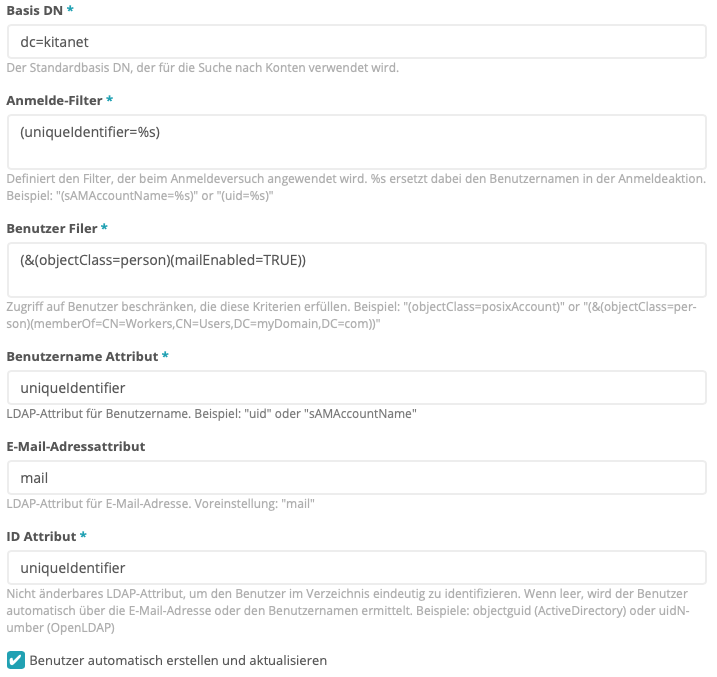
\includegraphics[width=1.0\textwidth]{res/ldapkitanet2.png}
  \caption{Teil 2 der LDAP-Konfiguration für Kitanet (Eigene Abbildung)}
  \label{fig:LDAP Kitanet Teil 2}
\end{figure}

Im unteren Teil der Einstellungen wird zunächst der \textit{Basis DN} festgelegt. Dieser legt fest in welchem Pfad des LDAP nach neuen Nutzern gesucht werden soll. Im hier vorliegenden Fall sollen zunächst alle Objekte erfasst werden, sie sich in der \ac{dn} \textit{kitanet} befinden.

Der \textit{Anmelde-Filter} legt fest, welches Attribut gegen den beim Login eingegebenen Nutzernamen geprüft wird. Dies steht auch in direkter Verbindung zu den Feldern \textit{Benutzernamen Attribut} und \textit{ID Attribut} die auch beide aus dem Attribut \textit{uid} ihre Informationen beziehen. 

Das Feld \textit{Benutzer Filer} legt fest, dass nur solche Objekte in Kitanet erfasst werden die ein Attribut namens \textit{objectClass} mit dem Wert \textit{posixAccount} besitzen.

Wichtig für die hier vorliegende Problemstellung ist noch die Verknüpfung der E-Mail-Adresse des Humhub-Nutzers mit dem LDAP-Attribut \textit{mail}. 

Das Auslesen des \ac{ldap} führt somit zu nachfolgender Nutzerliste.

\begin{figure}[h]
  \centering
  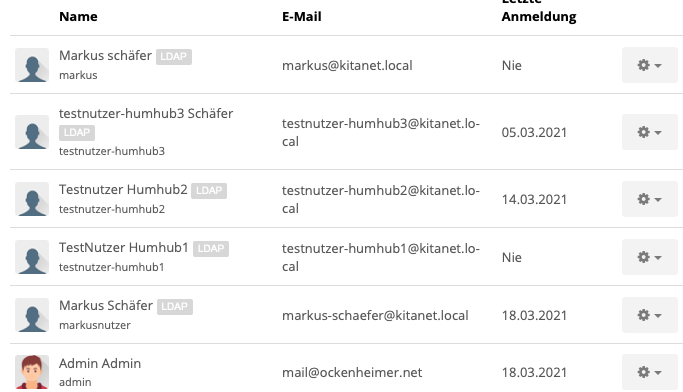
\includegraphics[width=1.0\textwidth]{res/nutzerliste.png}
  \caption{Nutzerliste der Testumgebung (Eigene Abbildung)}
  \label{fig:Nutzerliste}
\end{figure}

Das \ac{ldap} wird periodisch über einen sogenannten \textit{Cronjob} ausgelesen. Neue Nutzer werden entsprechend den oben dargestellten Kriterien angelegt und können sich ab diesem Moment mit dem in \ac{ldap} vergebenen Kennwort anmelden.

Dies schließt die Beschreibung des \textit{IST-Zustand} von Kitanet und der Testumgebung ab. Im folgenden sollen nun die Grundlagen zum E-Mail-Versand dargestellt werden.

\chapter{SMTP}
Was macht das \ac{smtp}? Beschreibung der Funktion von E-Mail

\textquote{The main purpose of SMTP is to deliver messages to user‘s mailboxes} \citep[][11]{rfc821}.

\chapter{Anforderungen/Nutzungsszenarien}
\section{Anforderungen}
Beschreibt die Anforderungen an den SMTP-Server, z.B.:
\begin{itemize}
	\item Lauffähig auf Ubuntu
	\item Zusammenarbeit mit LDAP
	\item Automatisierung der Nutzerverwaltung
	\item Gute Dokumentation
	\item geringer (im besten Fall gar kein) Wartungsaufwand
	\item Kostengünstig
	\item etc.
\end{itemize}


\section{Nutzungsszenarien}
Welche Szenarien soll der \ac{mta} abdecken? Welche Funktionen sind notwendig (\zb nur interne Mails, keine Erreichbarkeit von außen)? Was ist bei der Lizenzierung zu beachten? Gibt es weitere wichtige Aspekte? Der SMTP-Server soll mit dem eingesetzten IMAP-Client Dovecot zusammenarbeiten.
\section{Testfälle}
Aufgrund der beschriebenen Nutzungsszenarien werden Testfälle formuliert, die den Erfolg des Projektes kennzeichnen. 

\chapter{Zur Auswahl stehende SMTP-Software}
Vergleich von SMTP-Server-Software für den Einsatz auf Ubuntu. 
\section{postfix}
Erfüllt die Software die gestellten Anforderungen? Was spricht gegen einen Einsatz?
\section{EmailSuccess}
Inhaltlich wie oben.

\chapter{Entscheidung}
Welche SMTP-Software wurde gewählt? 

\chapter{Installation und Tests}

\section{Einrichtung und Anbindung SMTP an LDAP}
Wie steuert das \ac{ldap} den SMTP-Server? Wie funktioniert der Informationsaustausch (neue Nutzer, etc)?

\section{Tests}
Allgmeines zu den durchgeführten Tests. Kam es zu Problemen bei der Testung?
\subsection{Dokumenation der einzelnen Tests}
Wurde der Test bestanden? Musste der Test unerwartet an die Gegebenheiten angepasst werden?

\chapter{Fazit}

\blindtext
